\documentclass[10pt]{article}
\usepackage{graphicx}
\usepackage[margin=1.5cm]{geometry}
\usepackage{amsmath}
\def\brcurs{{\mbox{$\resizebox{.16in}{.08in}{
\includegraphics{BoldR}}$}}}
\def\rcurs{{\mbox{$\resizebox{.16in}{.08in}{
\includegraphics{ScriptR}}$}}}

\begin{document}
\twocolumn

\title{Tuesday Warm-up: Electrostatics}
\author{Prof. Jordan C. Hanson}

\maketitle

\section{Memory Bank}

\begin{itemize}
\item Permittivity of free space: $\epsilon_0 = 8.85 \times 10^{-12}$ N$^{-1}$C$^2$m$^{-2}$
\item Coulomb's Law, discrete
\begin{equation}
\mathbf{E}(\mathbf{r}) = \frac{1}{4\pi\epsilon_0}\sum_i \frac{q_i}{\rcurs_i^2}\hat{\brcurs}
\end{equation}
\item Coulomb's Law, continuous
\begin{equation}
\mathbf{E}(\mathbf{r}) = \frac{1}{4\pi\epsilon_0}\int \frac{\rho(\mathbf{r}')}{\rcurs^2}\hat{\brcurs}d\tau'
\end{equation}
\end{itemize}

\begin{figure}
\centering
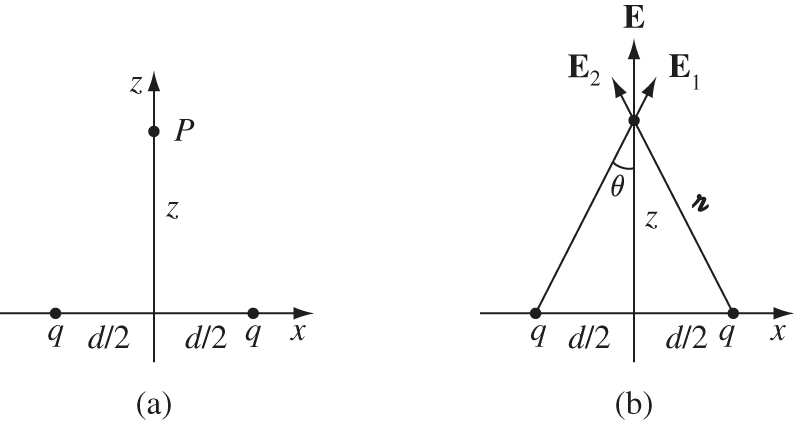
\includegraphics[width=0.4\textwidth]{figures/2_4.jpg}
\caption{\label{fig:1} A dipole of two positive charges.}
\end{figure}

\section{Discrete Charge Distributions}

\begin{enumerate}
\item Consider Fig. \ref{fig:1}.  Find the electric field a distance $z$ above the midpoint between two equal charges $q$ a distance $d$ apart. Check that the units are N C$^{-1}$.  \\ \vspace{3cm}
\item (a) Using the result from exercise 1, take the following limits: (i) $z\gg d$ (ii) $z\to 0$. (b) How would the calculation change if the charge at $(d/2)\hat{i}$ was negative? \\ \vspace{1cm}
\item Consider Fig. \ref{fig:2}.  Suppose that, when viewing the square from $P$, there is a charge $-q$ at the lower right corner, a charge $q$ at the upper right corner, a charge $-q$ at the upper left corner, and a charge $q$ at the lower left corner.  Find the electric field at $P$. \\ \vspace{2.5cm}
\end{enumerate}

\begin{figure}
\centering
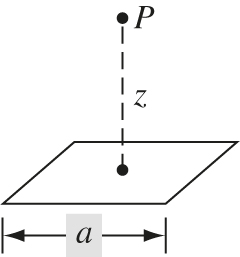
\includegraphics[width=0.15\textwidth]{figures/2_8.jpg}
\caption{\label{fig:2} A square of size $a$ in the xy-plane centered at the origin.  The point $P$ is a distance $z$ above the origin.}
\end{figure}
\begin{figure}
\centering
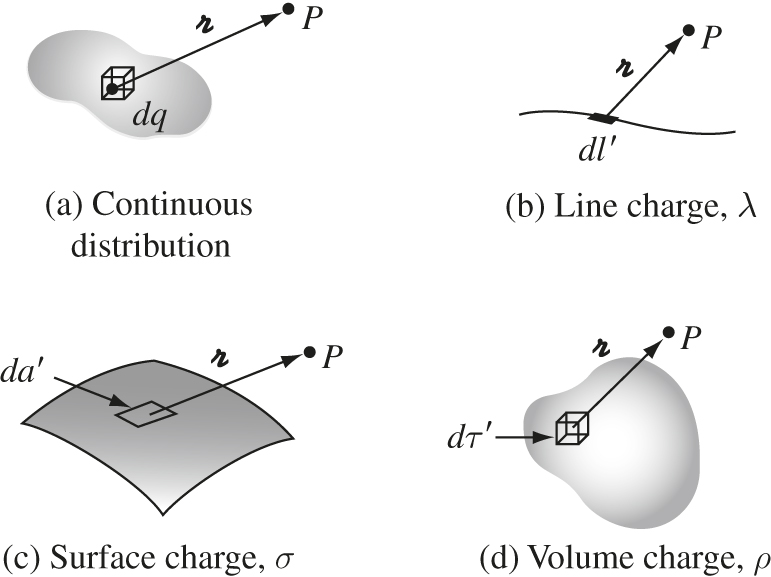
\includegraphics[width=0.4\textwidth,trim=0cm 3cm 0cm 0cm,clip=true]{figures/2_5.jpg}
\caption{\label{fig:3} Charge distributions each have a unique $dq$.}
\end{figure}

\section{Continuous Charge Distributions}

\begin{enumerate}
\item Consider Fig. \ref{fig:1}. Suppose that instead the $q$ was spread uniformly between $[-d/2, d/2]$, with a density $\lambda$ (C m$^{-1}$). Find the electric field a distance $z$ above the midpoint.
\end{enumerate}

\end{document}
